\documentclass[letterpaper,12pt]{article}

% Import packages from .sty file.
%\usepackage{imports}

% Mike's things because he couldn't figure out how to get the preamble working otherwise
\usepackage[utf8]{inputenc}
\usepackage{geometry,ulem,graphicx,caption,color,setspace,dsfont,amssymb}
\usepackage[comma]{natbib}
\usepackage{subcaption} 
\usepackage[short]{optidef}
\usepackage{hhline}
\usepackage[capposition=top]{floatrow}
\usepackage{booktabs} % Allows the use of \toprule, \midrule and \bottomrule in tables
\usepackage{adjustbox}
\usepackage{tikz}
\usepackage{pdflscape}
\usetikzlibrary{calc,patterns,positioning}
\usepackage{environ}
\usepackage{soul}

\bibliographystyle{ecta}

\usepackage{titlesec}
\titleformat{\section}
  {\normalfont\normalsize\bfseries}{\thesection.}{1em}{}

\titleformat{\subsection}
  {\normalfont\normalsize\bfseries}{\thesubsection}{1em}{}


%%%%%%%%%%%%%%%%%%%%%%%%%%%%%%%%%%%%%%%%%%%%%%%%%%%%%%%%%%%%%%%%%
%%%%%%%%%%%%%%%%%%%%%%%%%%%%% Title %%%%%%%%%%%%%%%%%%%%%%%%%%%%%
%%%%%%%%%%%%%%%%%%%%%%%%%%%%%%%%%%%%%%%%%%%%%%%%%%%%%%%%%%%%%%%%%

\begin{document}

\begin{center}
    \noindent \textbf{From Value Added to Welfare Added}
\end{center}




%%%%%%%%%%%%%%%%%%%%%%%%%%%%%%%%%%%%%%%%%%%%%%%%%%%%%%%%%%%%%%%%%
%%%%%%%%%%%%%%%%%%%%%%%%%%%% Project %%%%%%%%%%%%%%%%%%%%%%%%%%%%
%%%%%%%%%%%%%%%%%%%%%%%%%%%%%%%%%%%%%%%%%%%%%%%%%%%%%%%%%%%%%%%%%

\section{Project Description}

Education policies seeking to promote teacher accountability typically have specific distributional goals for students. For example, some focus on minority groups, low-achieving students, or other at-risk populations. Furthermore, these policies often use value added measures (VAM) to evaluate and compare teachers in order to better promote various policy goals. Though VAM seem to perform well in the face of possible biases and capture real information about the long-term effects that teachers have on students \citep{chetty2014measuring1, chetty2014measuring2}, there seems to be a philosophical disconnect between these distributional goals and tradition VAM. This disconnect comes because VAM are mean oriented statistics and are thus completely utilitarian. In this project we seek to bridge this disconnect by proposing a set of more flexible measures that allow for heterogeneity in teacher value added across the achievement distribution.

In particular, we explore using standard value added including bins for prior achievement, quantile regression, and kernel regression to estimate the value added for each teacher. We then run Monte Carlo simulations to compare each of these estimators to standard value added. We will evaluate each by how well they recover the true, welfare weighted ranking of teachers (i.e. which teachers contribute the greatest value added weighted by the policy maker's explicit welfare weights) and by how well each performs in a single sample. These simulations will also allow us to understand whether these more flexible measures are feasible given the data constraints in real-world settings.

We are also working to acquire administrative student-teacher linked data, with which we will be able to explore questions such as "what gains might we expect if teachers and students were better matches?" or "what are the costs in terms of the states policy goals for using standard VAM as opposed to our more flexible measures?"




%%%%%%%%%%%%%%%%%%%%%%%%%%%%%%%%%%%%%%%%%%%%%%%%%%%%%%%%%%%%%%%%%
%%%%%%%%%%%%%%%%%%%%%%%%%%% Simulation %%%%%%%%%%%%%%%%%%%%%%%%%%
%%%%%%%%%%%%%%%%%%%%%%%%%%%%%%%%%%%%%%%%%%%%%%%%%%%%%%%%%%%%%%%%%

\section{Simulation}

We have built simulations with the following features:

\begin{enumerate}
    \item Students are drawn from a particular `ability' distribution (e.g. standard normal).
    \item Teachers are given a random ability (i.e. the average level of test score improvement they help students achieve) and a random center (i.e. the part of the achievement distribution they are best at teaching, standard normally distributed but capped at -2 and 2). See the black dots in Figure \ref{fig:teacher_ex} for an example of a teacher with ability 0 and center ~1.2.
    \item We vary the level of heterogeneity (e.g. the height of the spike in Figure \ref{fig:teacher_ex}.
    \item Students are assigned to teachers either randomly or with correlation between teacher and student ability, depending on the simulation.
    \item We can include linear-in-means peer effects.
    \item We have a variety of possible true teacher impact functions, for example see the black dots in Figure \ref{fig:teacher_ex}.
    \item In the future we hope to calibrate the amount of noise in various parameters to actual administrative data.
    \item We specify a particular weighting function for each simulation (e.g. rawlsian weights with .8 weight below the 40th percentile and .2 weight above).
\end{enumerate}


\begin{figure}[ht]
    \centering
    \caption{Example Teacher Impact Figure with Estimated Impact}
    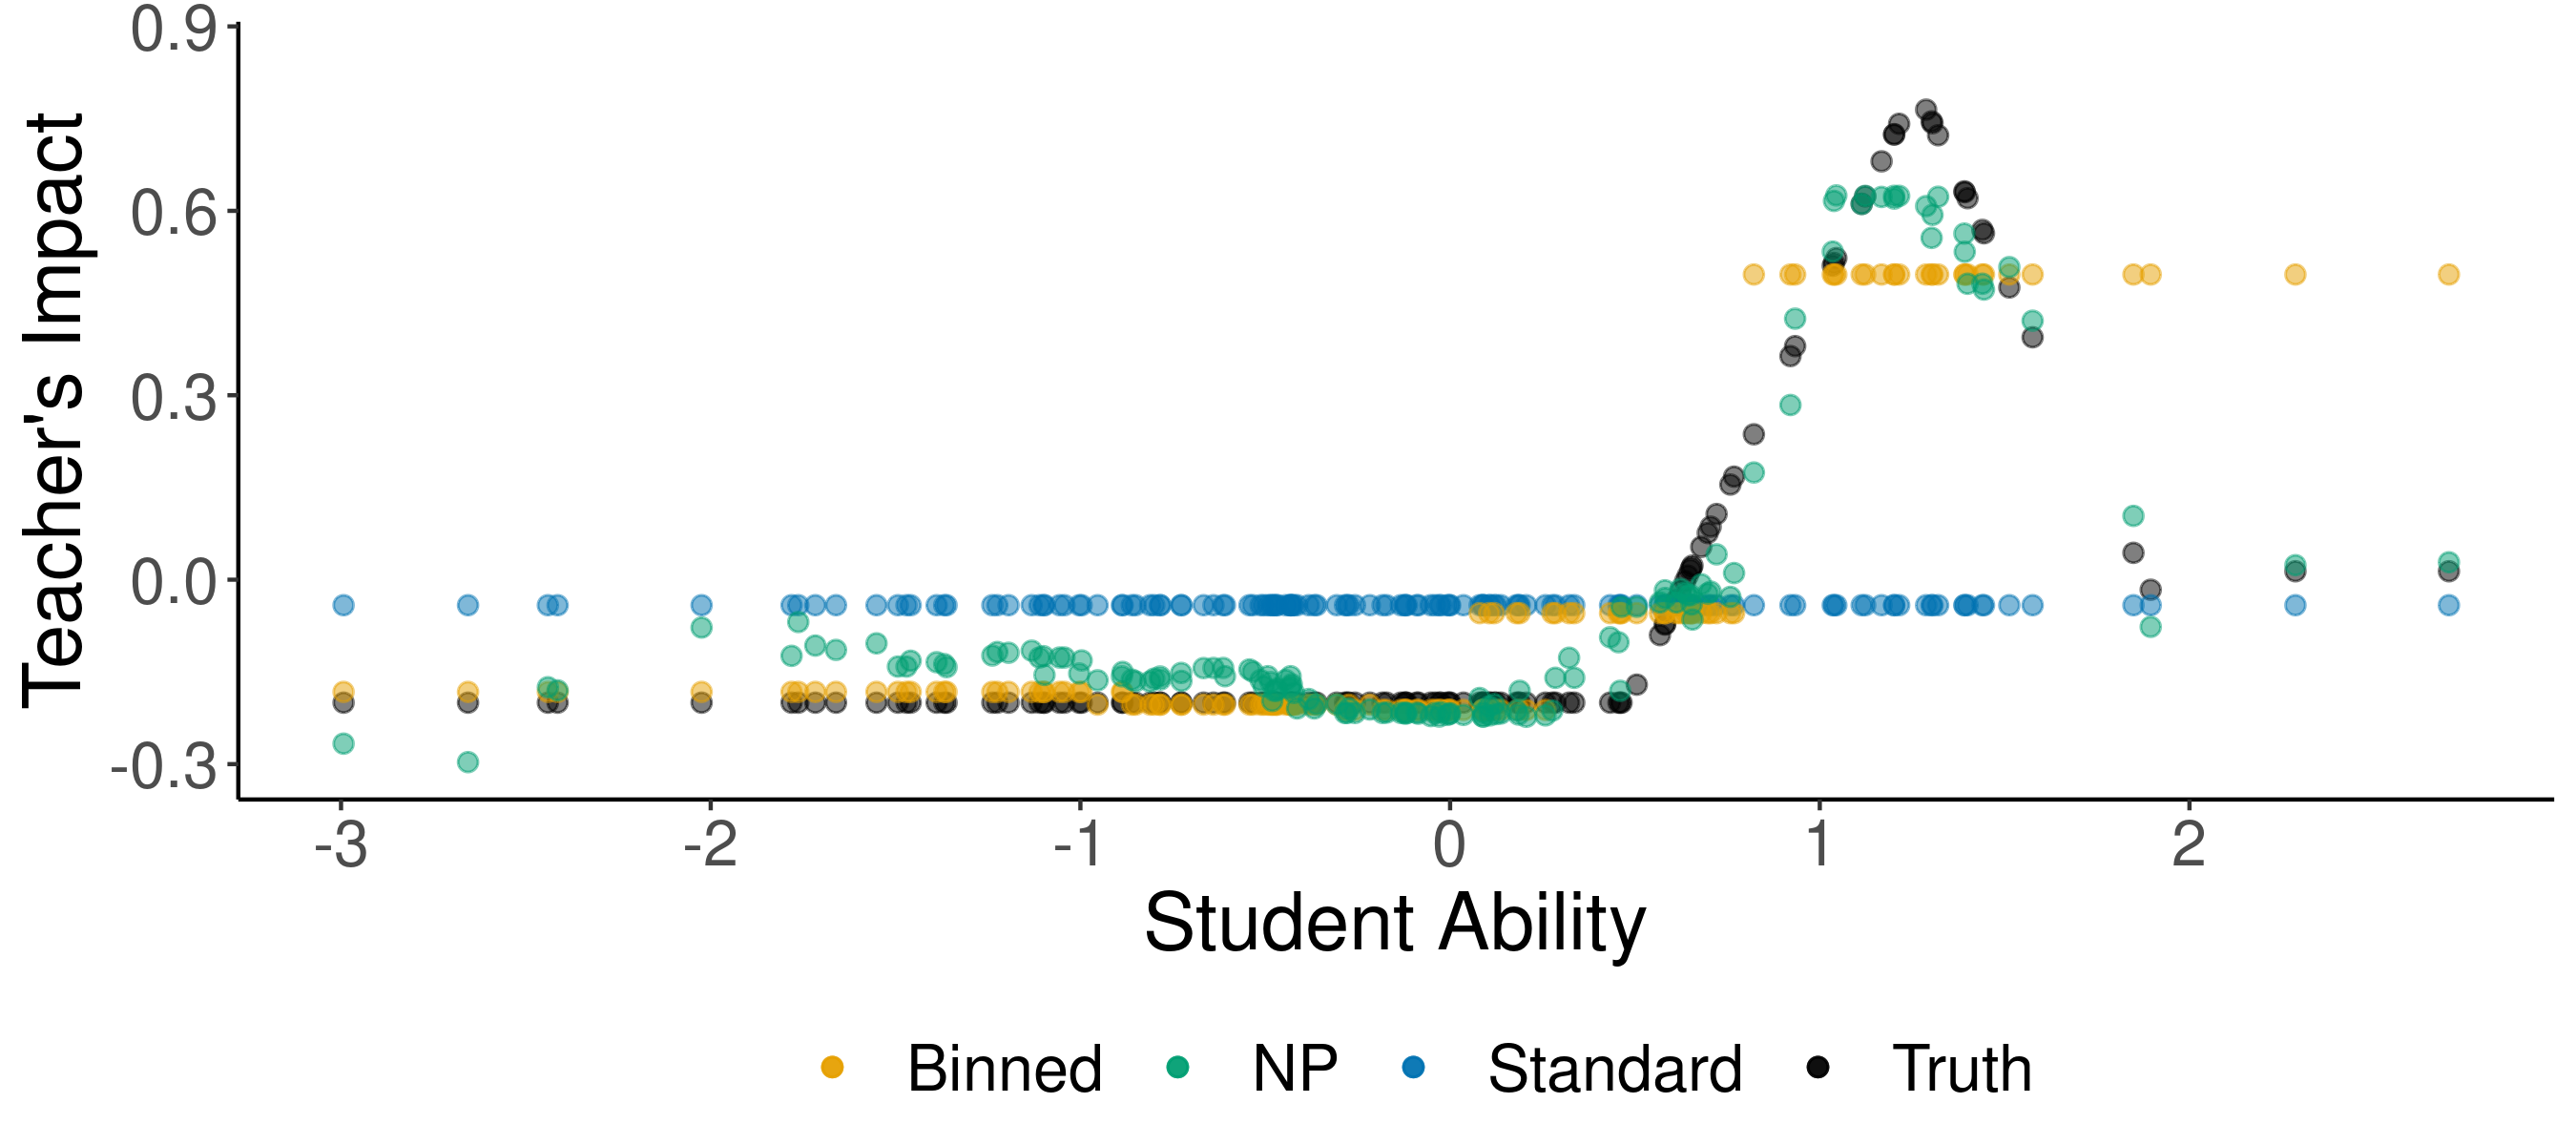
\includegraphics[width=.9\textwidth]{slides/CIERS_Figures/teacher_example_1.png}
    \label{fig:teacher_ex}
\end{figure}

Here are a few example simulations. The first set of figures are from a clearly unrealistic simulation that we feel gives good intuition for the situation. In this simulation we have no variation in teacher ability, only variation in teacher center, so the only difference between teachers is which students they excel at teaching. We also use rawlsian weights with .8 weight below the 40th percentile and .2 weight above. The blue dots (which you can see well in Figure \ref{fig:stand_cat} but not so much in Figure \ref{fig:alt_cat}) show the true (potential) impact for each teacher on the population of students (i.e. hypothetically if that teacher were to teach all students in the population what would their welfare weighted impact be), sorted lowest to highest. The pink dots in each figure then show the estimated impact using standard VA (Figure \ref{fig:stand_cat}) or kernel regression (Figure \ref{fig:alt_cat}). The standard VA is getting the rank order of teachers systematically wrong, and Figure \ref{fig:stand_cent} demonstrates why. The policy is using rawlsian weights, so cares much more about students below the 40th percentile in the achievment distribution. However, she also cares about helping more students, so the teacher who best increases weighted welfare is the teacher who teaches well for a lot of students (i.e. has a center in the densest portions of the student distribution) and who teaches well for students the policy maker cares more about (those under the 40th percentile). Standard VA is only for teachers who have centers in high density areas, and this is why the blue dots are shifted left from the pink dots.

\begin{figure}[ht]
    \centering
    \caption{True Welfare-Weighted Teacher Impact versus Standard VA Estimates}
    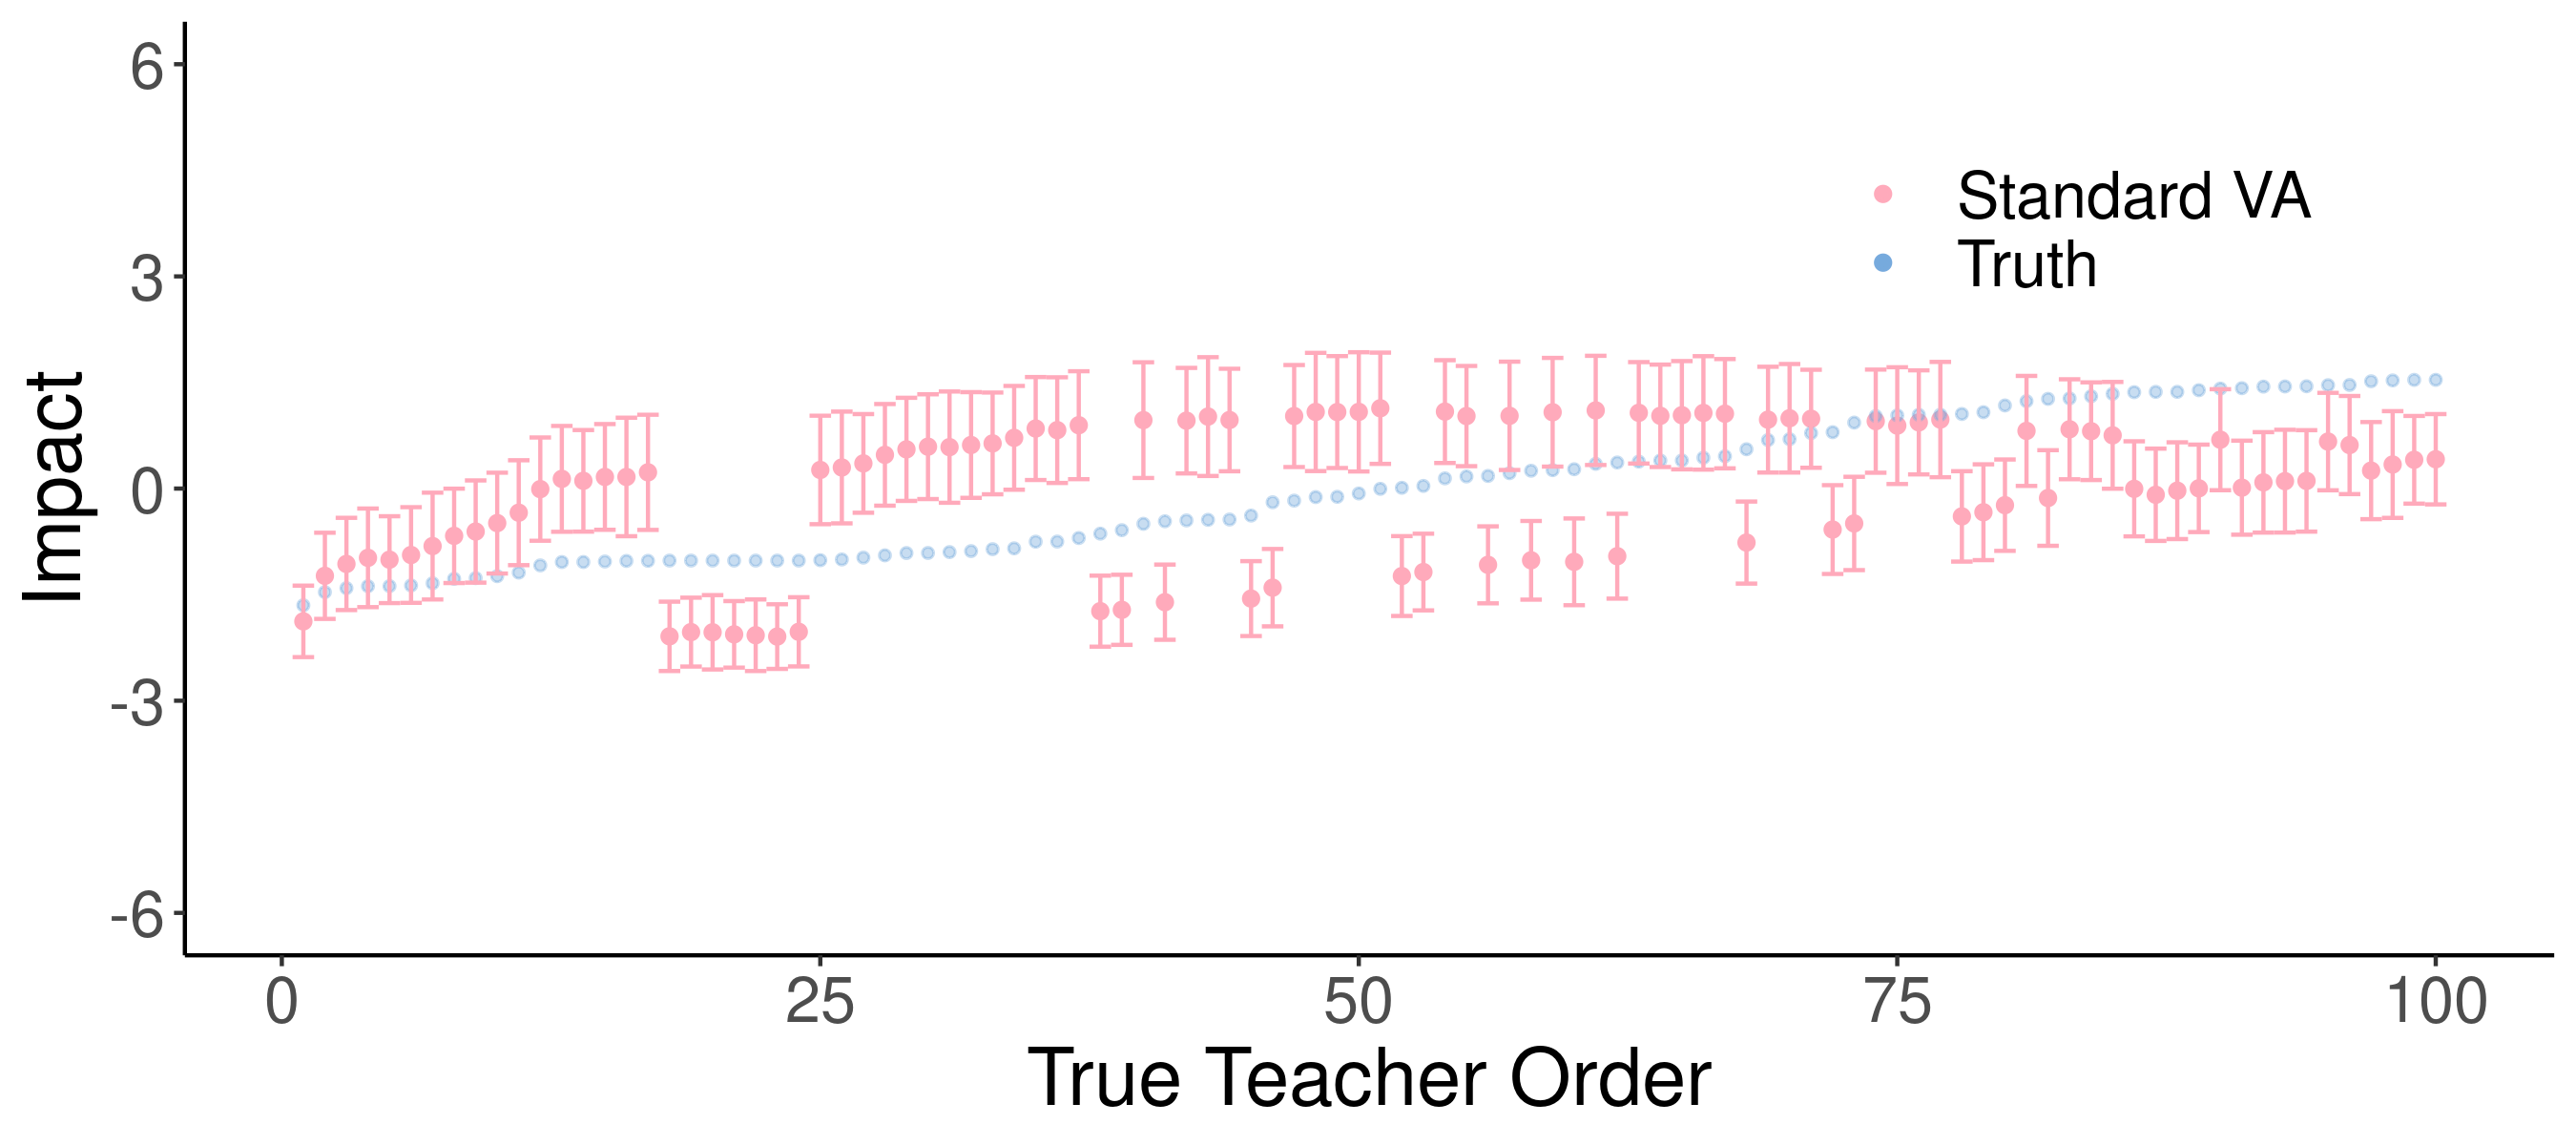
\includegraphics[width=.9\textwidth]{slides/CIERS_Figures/standard_cat_run_2.png}
    \label{fig:stand_cat}
\end{figure}

\begin{figure}[ht]
    \centering
    \caption{True Welfare-Weighted Teacher Impact versus Kernel Regression Estimates}
    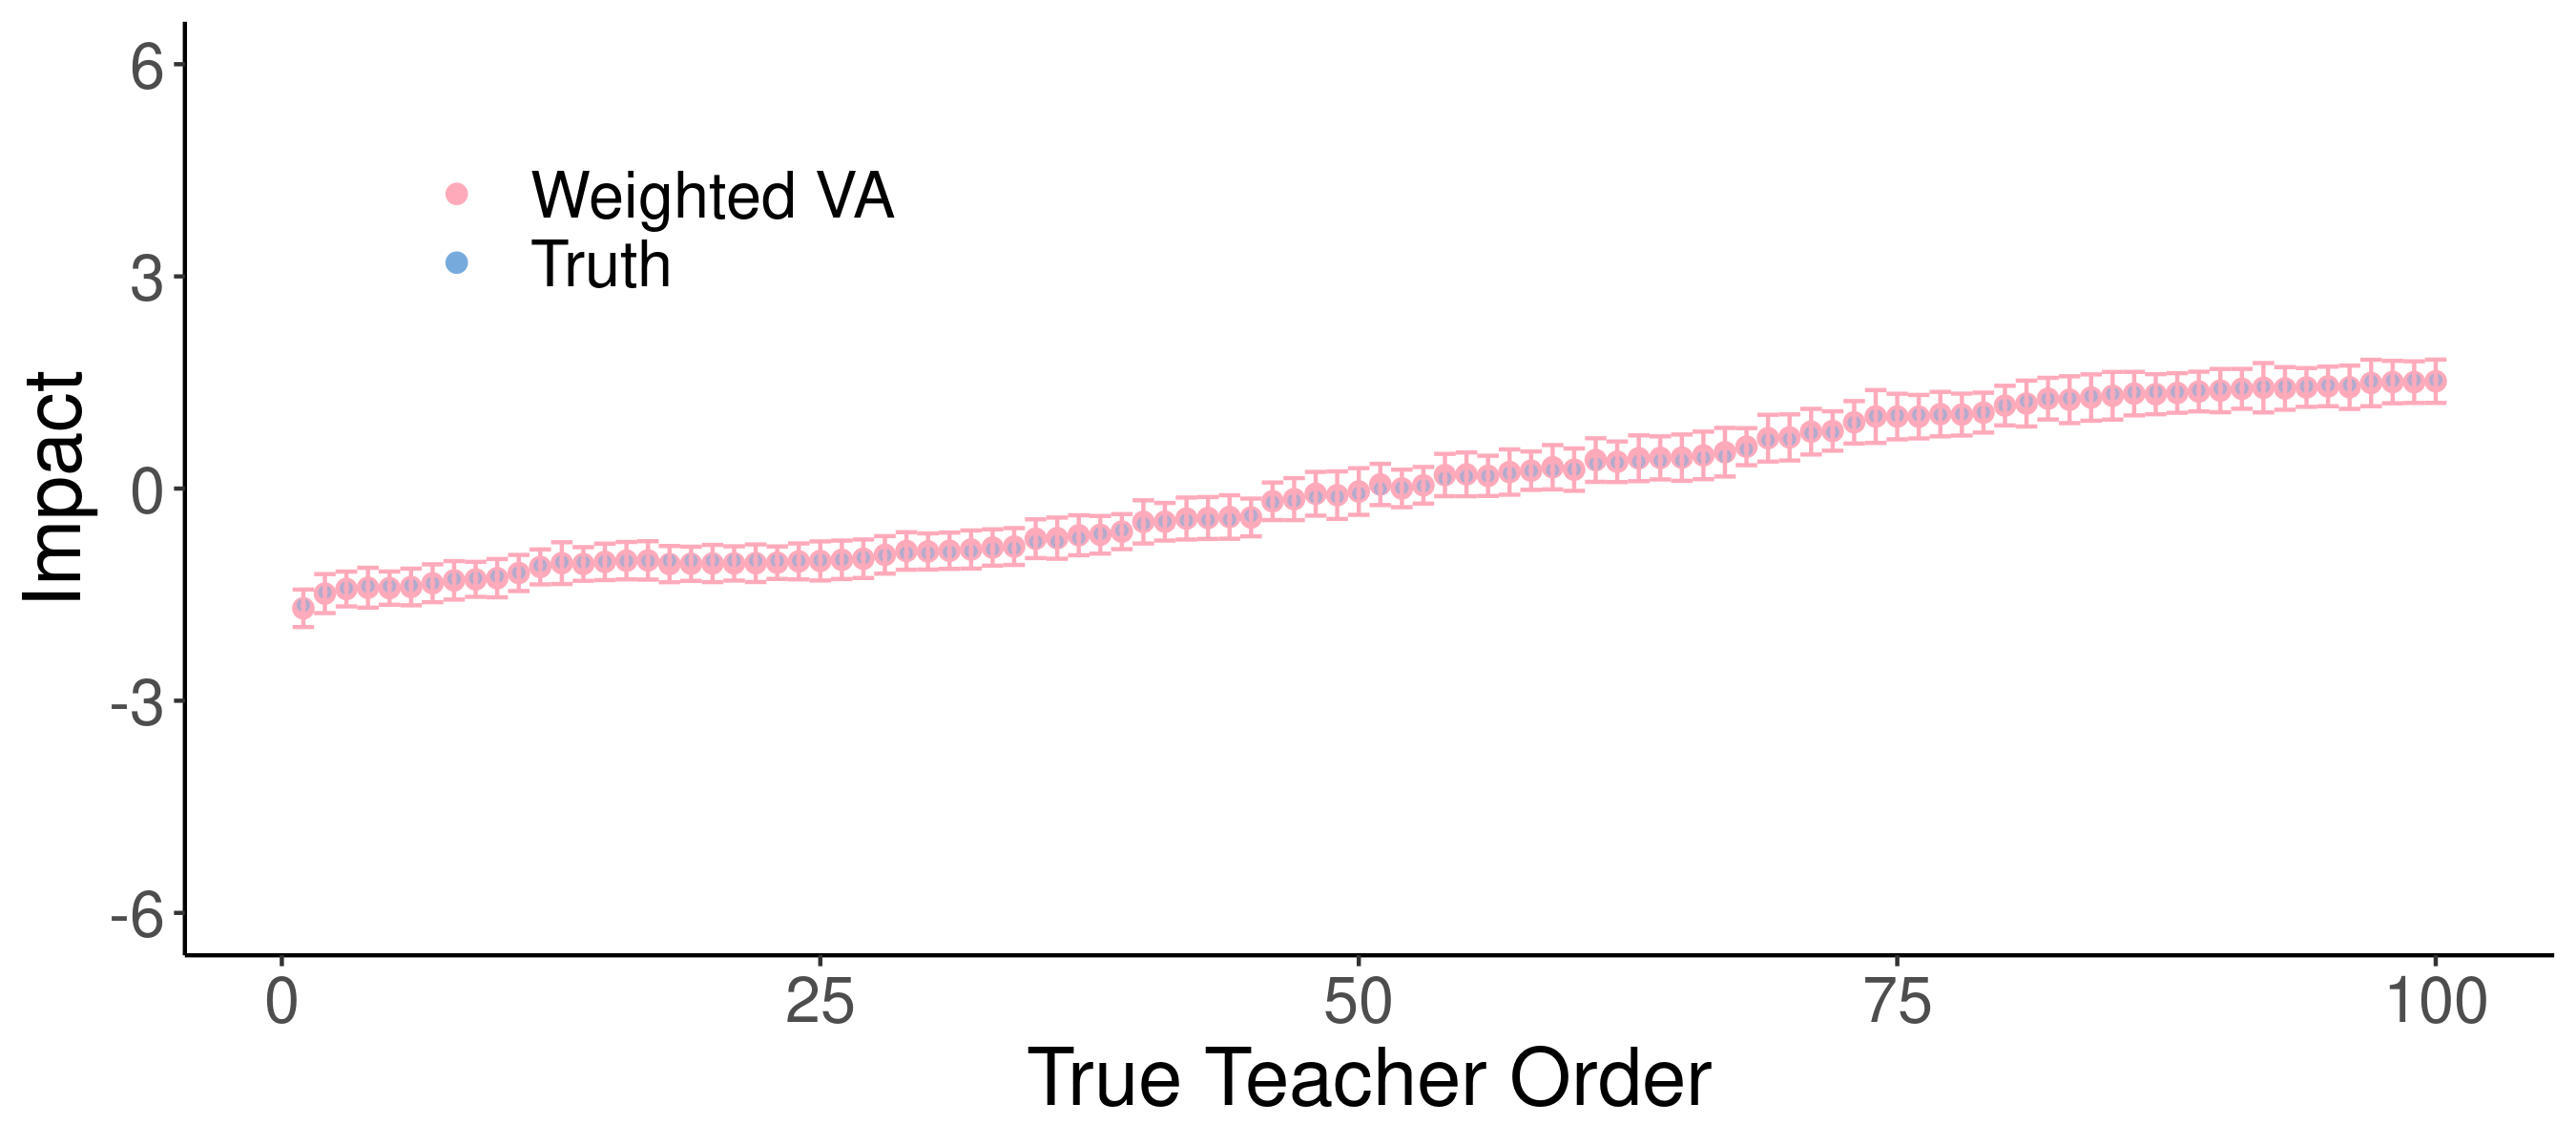
\includegraphics[width=.9\textwidth]{slides/CIERS_Figures/ww_cat_run_2.png}
    \label{fig:alt_cat}
\end{figure}

\begin{figure}[ht]
    \centering
    \caption{Estimated and True Impact Ordered by Teacher Center}
    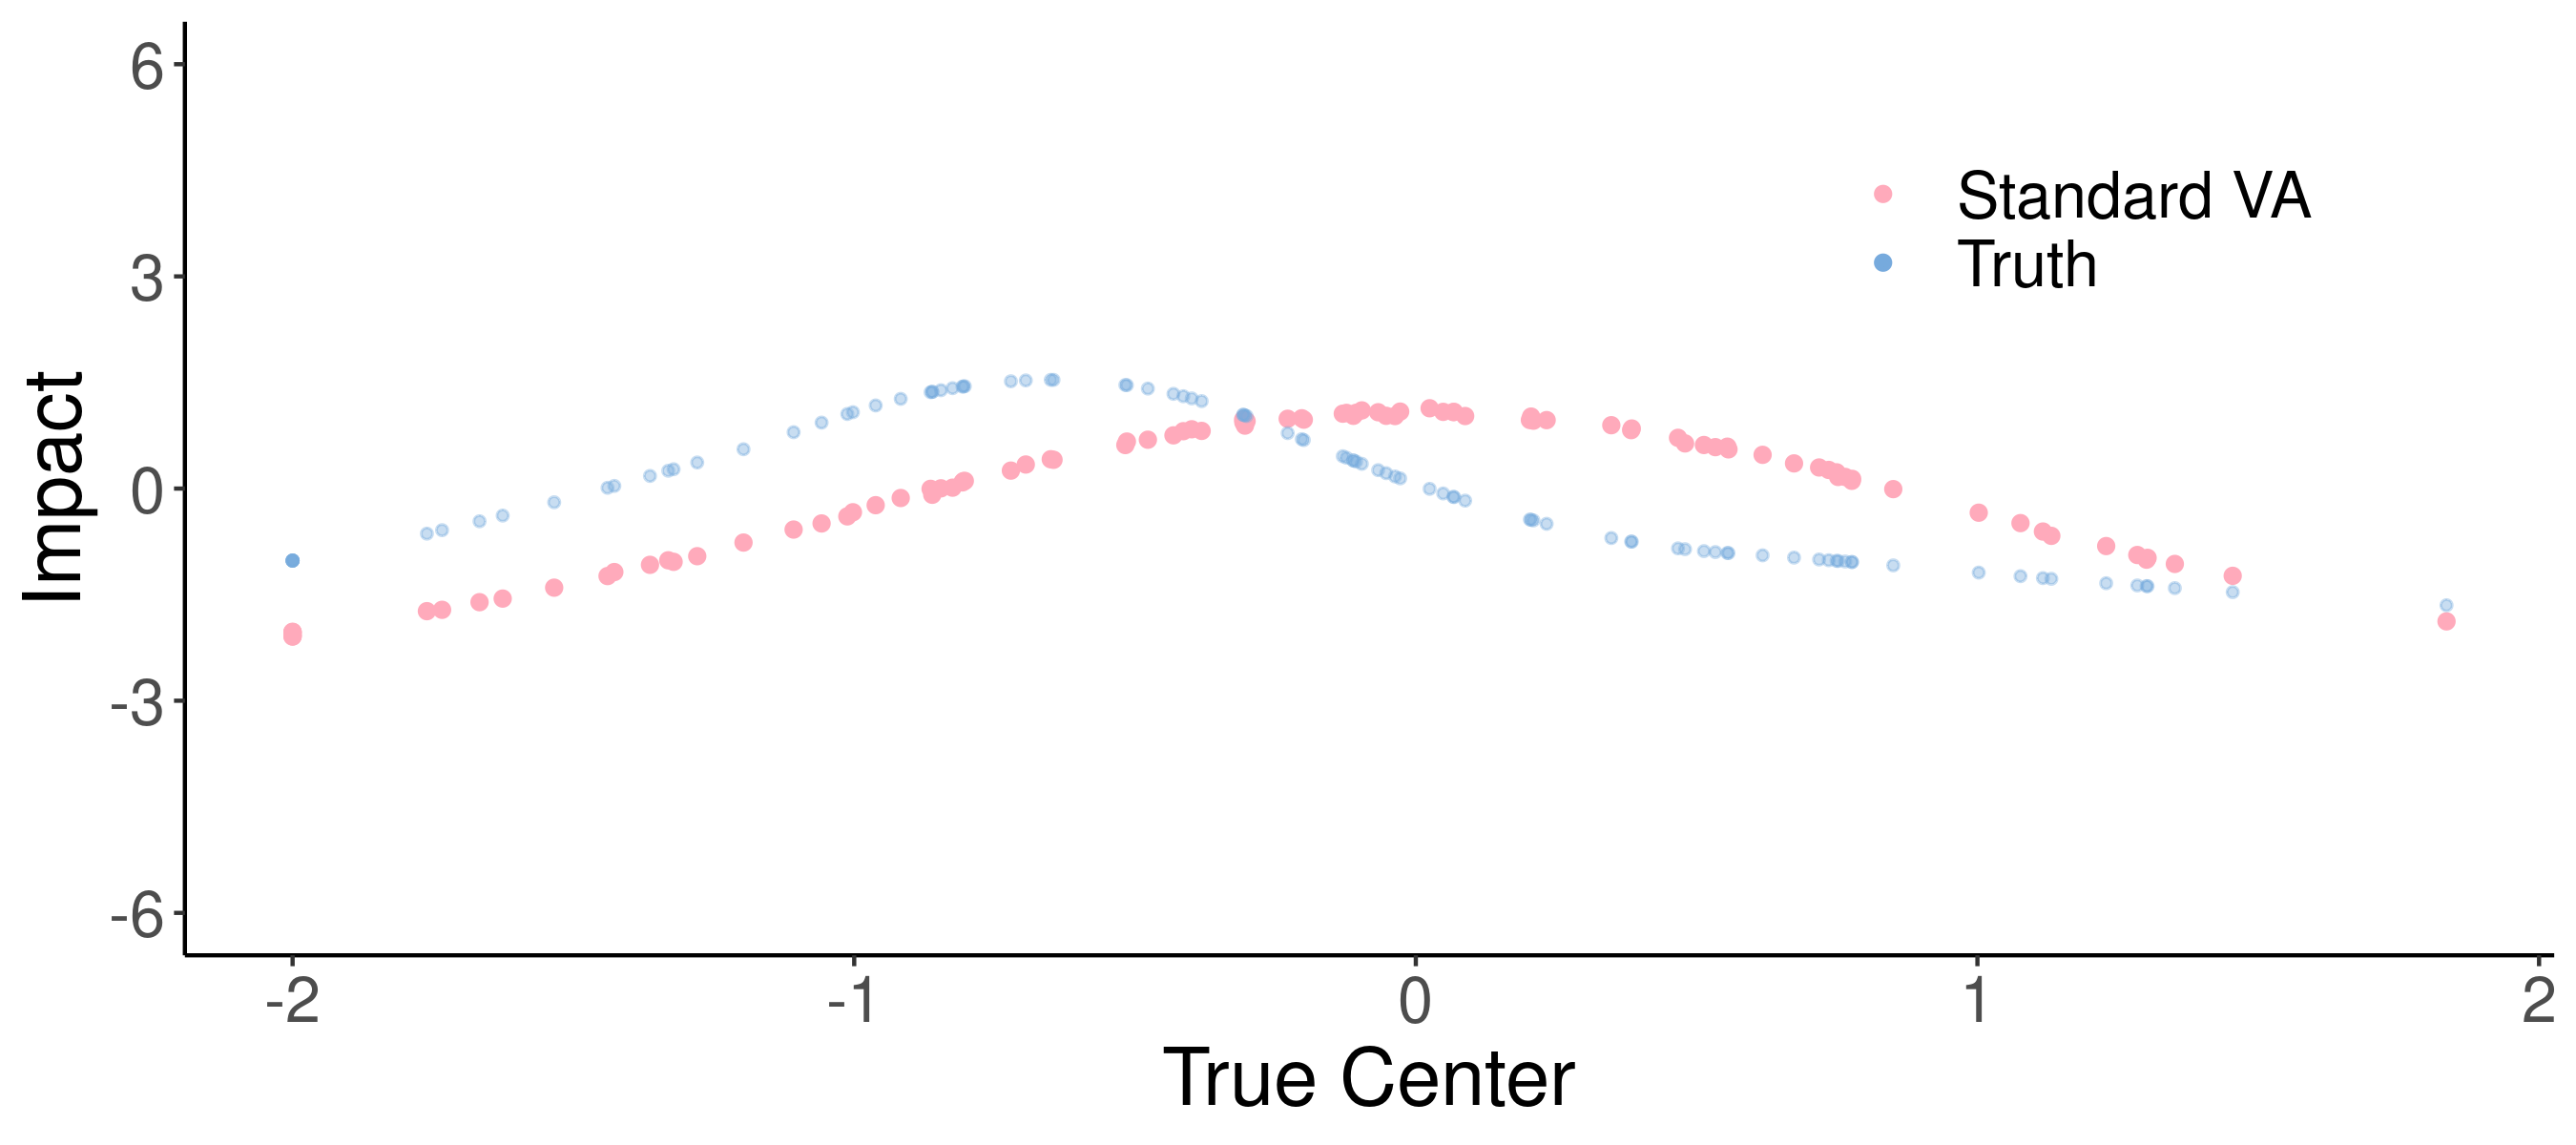
\includegraphics[width=.9\textwidth]{slides/CIERS_Figures/standard_cent_run_2.png}
    \label{fig:stand_cent}
\end{figure}

\begin{figure}[ht]
    \centering
    \caption{Estimated and True Impact Ordered by Teacher Center}
    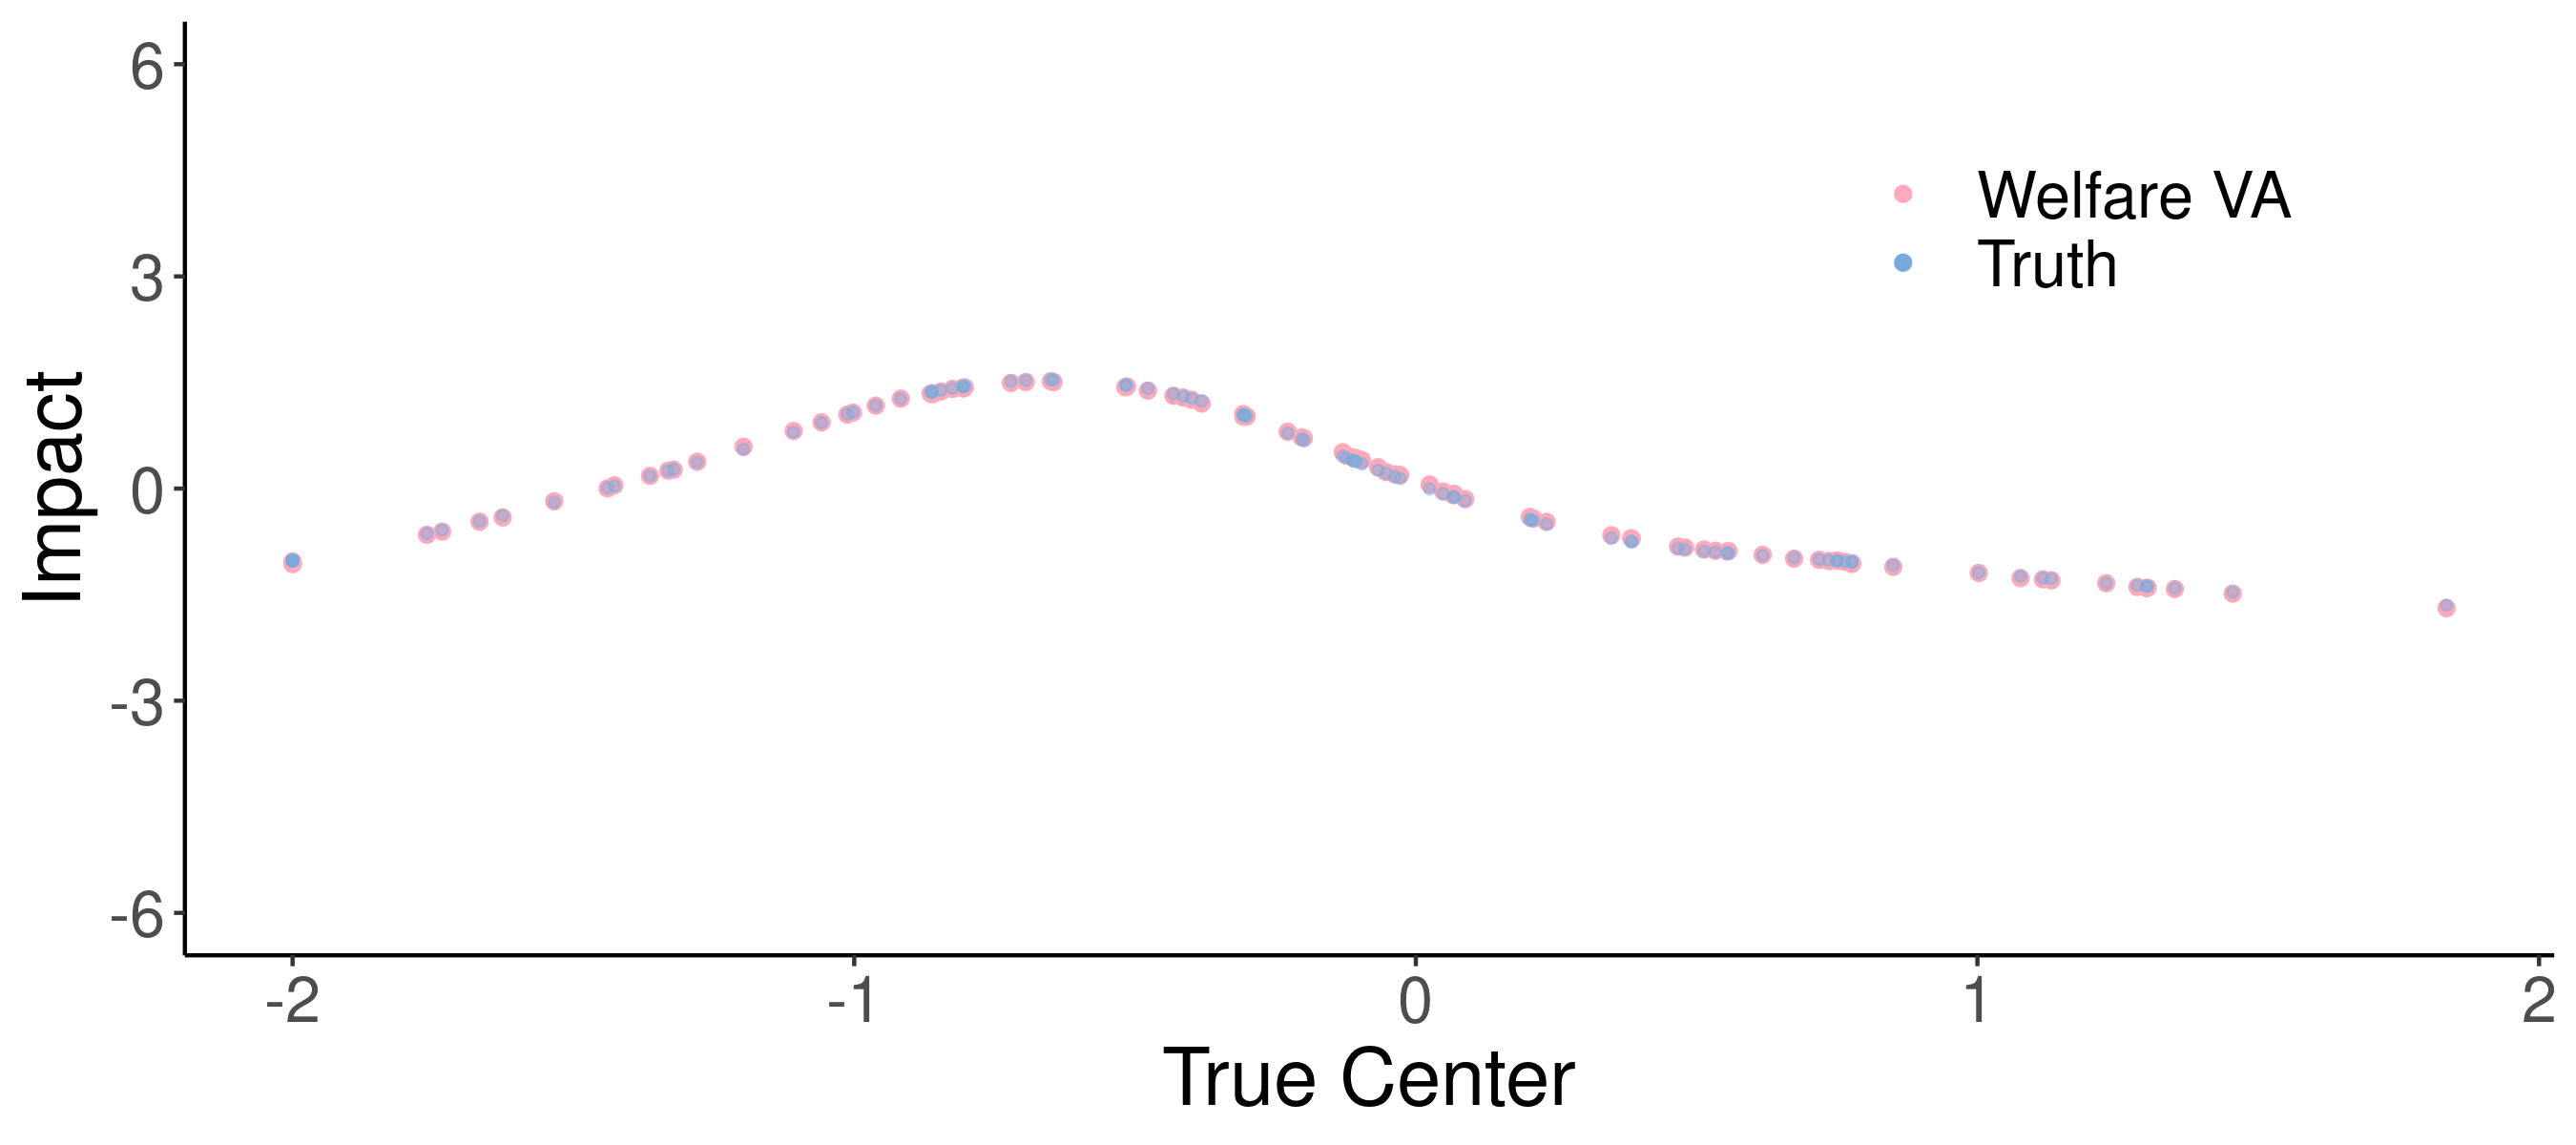
\includegraphics[width=.9\textwidth]{slides/CIERS_Figures/welfare_cent_run_2.png}
    \label{fig:alt_cent}
\end{figure}

This example is clearly a caricature, but if we allow for variance in teacher ability, peer effects, and student sorting but still have a reasonable amount of heterogeneity in teacher match the kernel regression still performs better (see Figures \ref{fig:stand_cat10} - \ref{fig:hist}). The standard VA and kernel regression are much closer here, but Figure \ref{fig:hist} shows that the mean rank difference is smaller for the kernel and the rank correlation to the true ranking is higher.

\begin{figure}[ht]
    \centering
    \caption{More Realistic Simulation, Standard VA}
    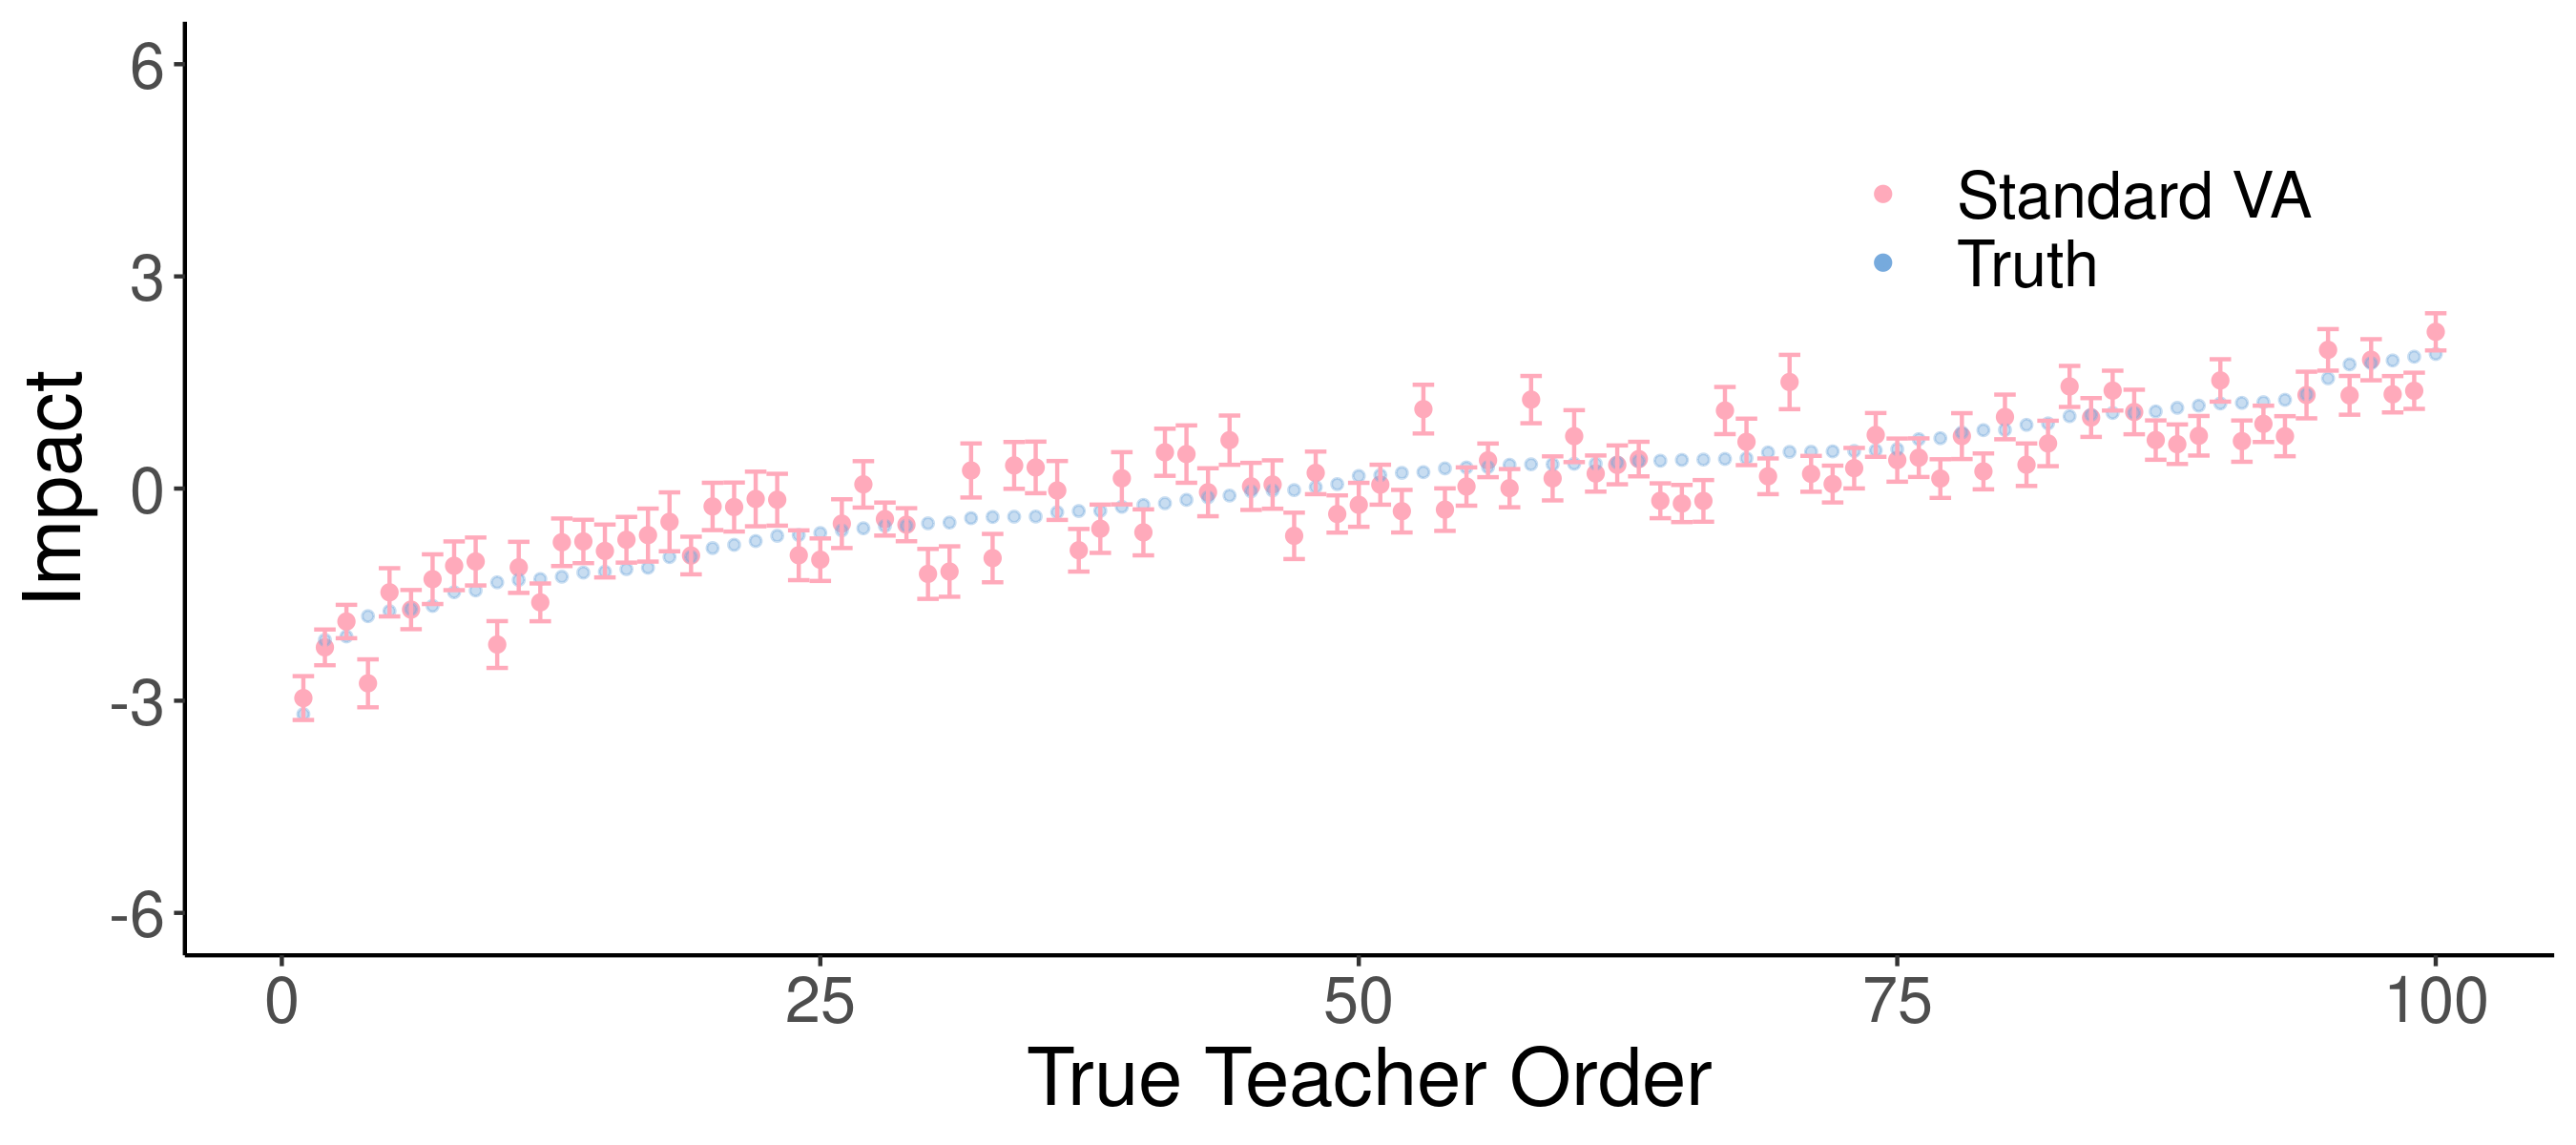
\includegraphics[width=.9\textwidth]{slides/CIERS_Figures/standard_cat_run_2_new.png}
    \label{fig:stand_cat10}
\end{figure}

\begin{figure}[ht]
    \centering
    \caption{More Realistic Simulation, Kernel Regression}
    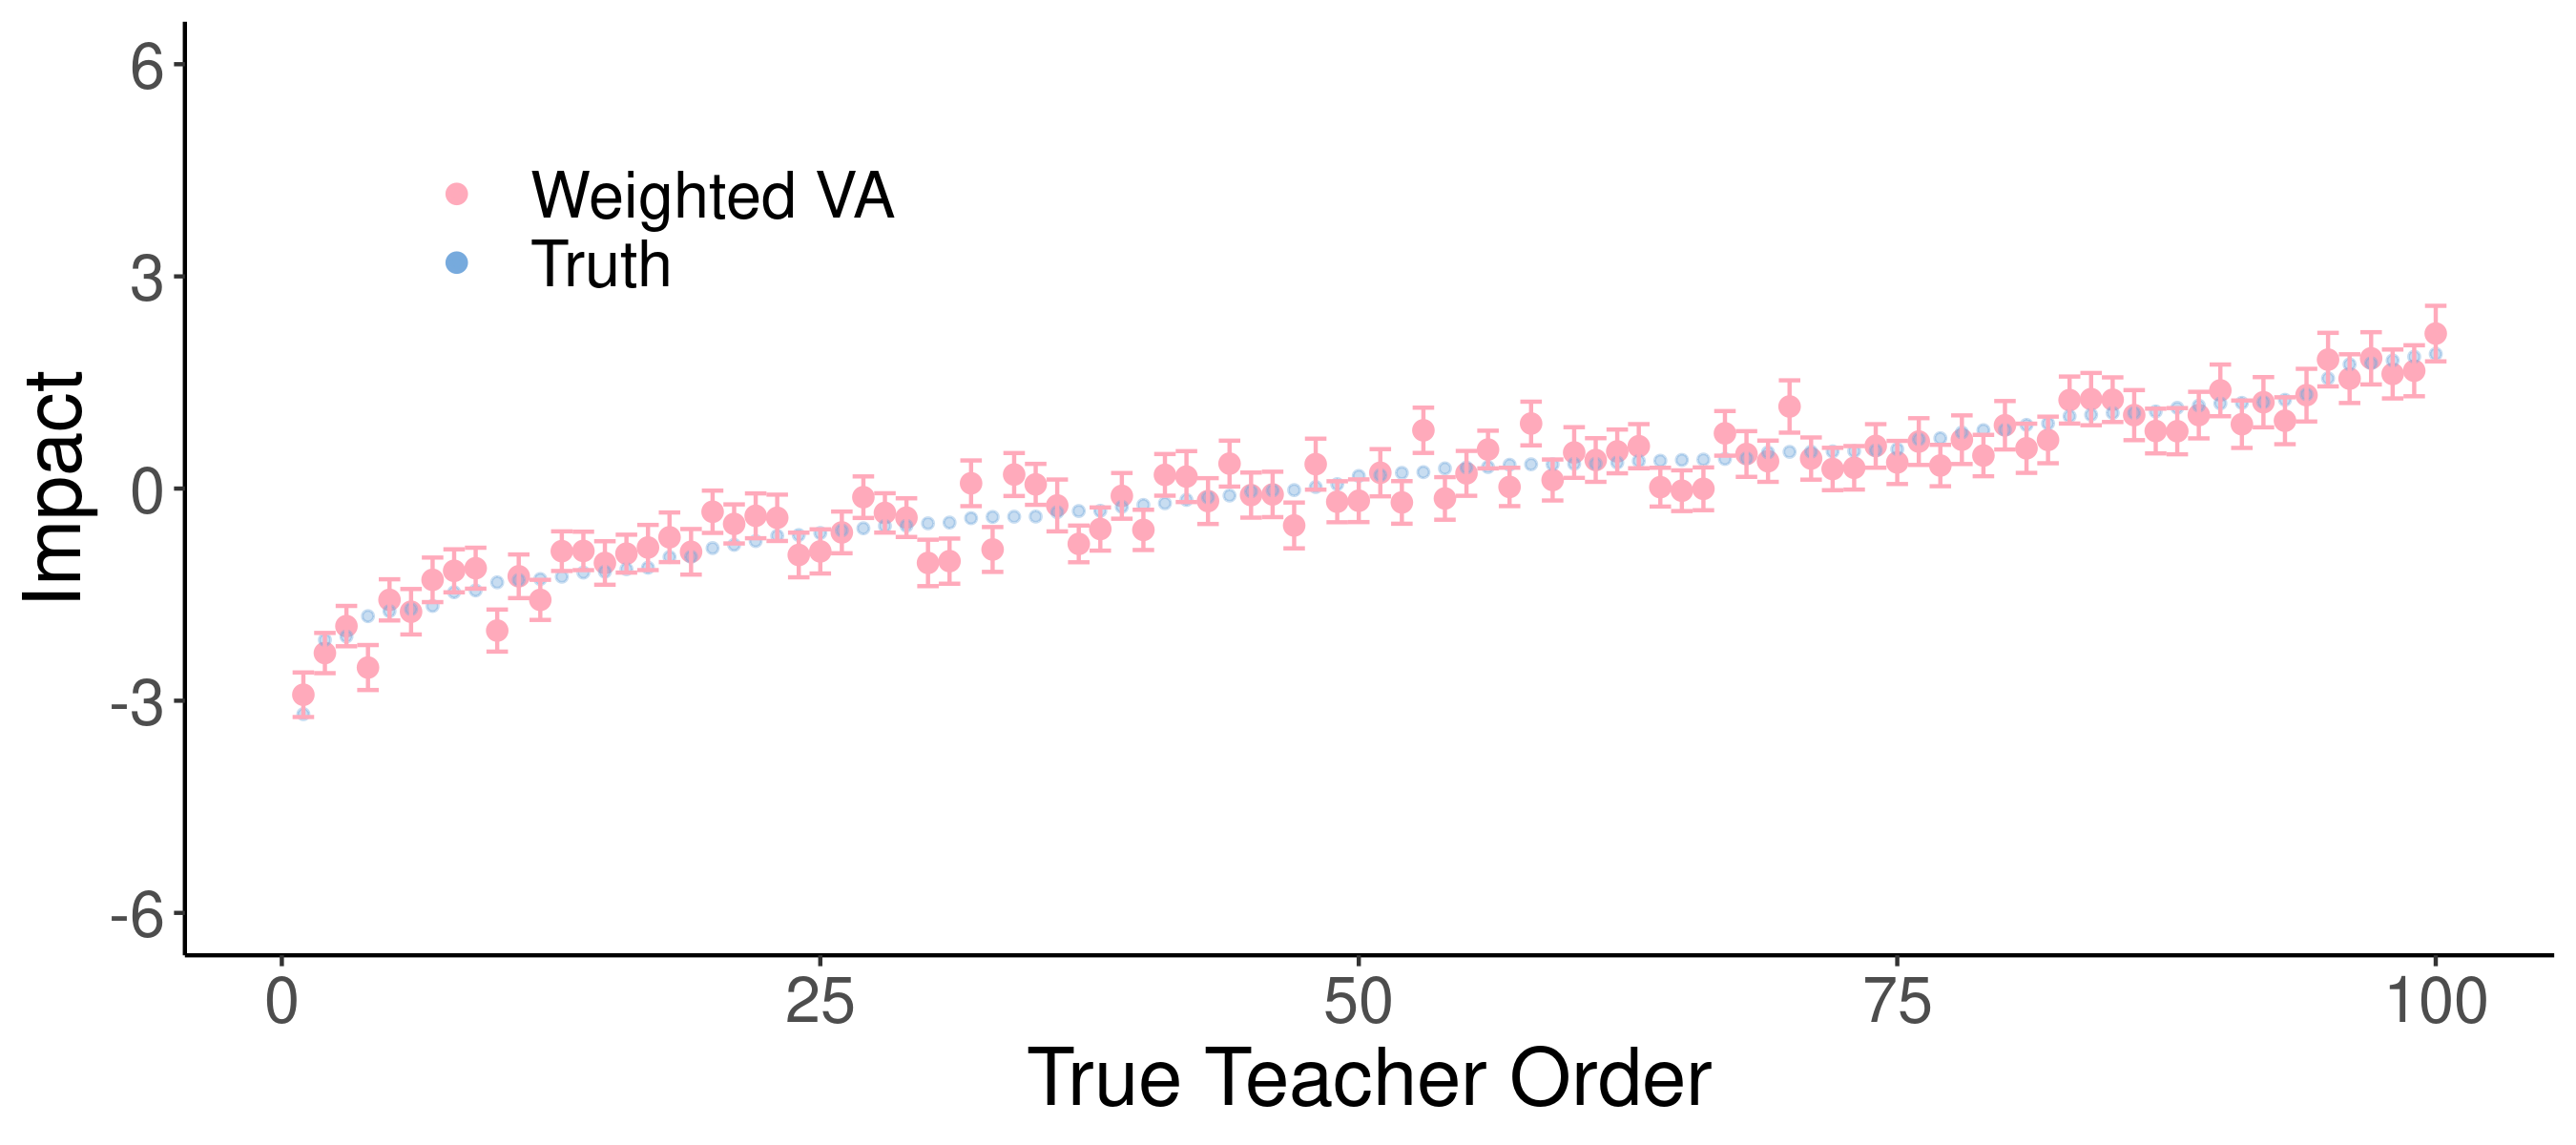
\includegraphics[width=.9\textwidth]{slides/CIERS_Figures/np_ww_cat_run_2.png}
    \label{fig:alt_cat10}
\end{figure}

\begin{figure}[ht]
    \centering
    \caption{More Realistic Simulation, Difference Between True and Estimated Rank Order}
    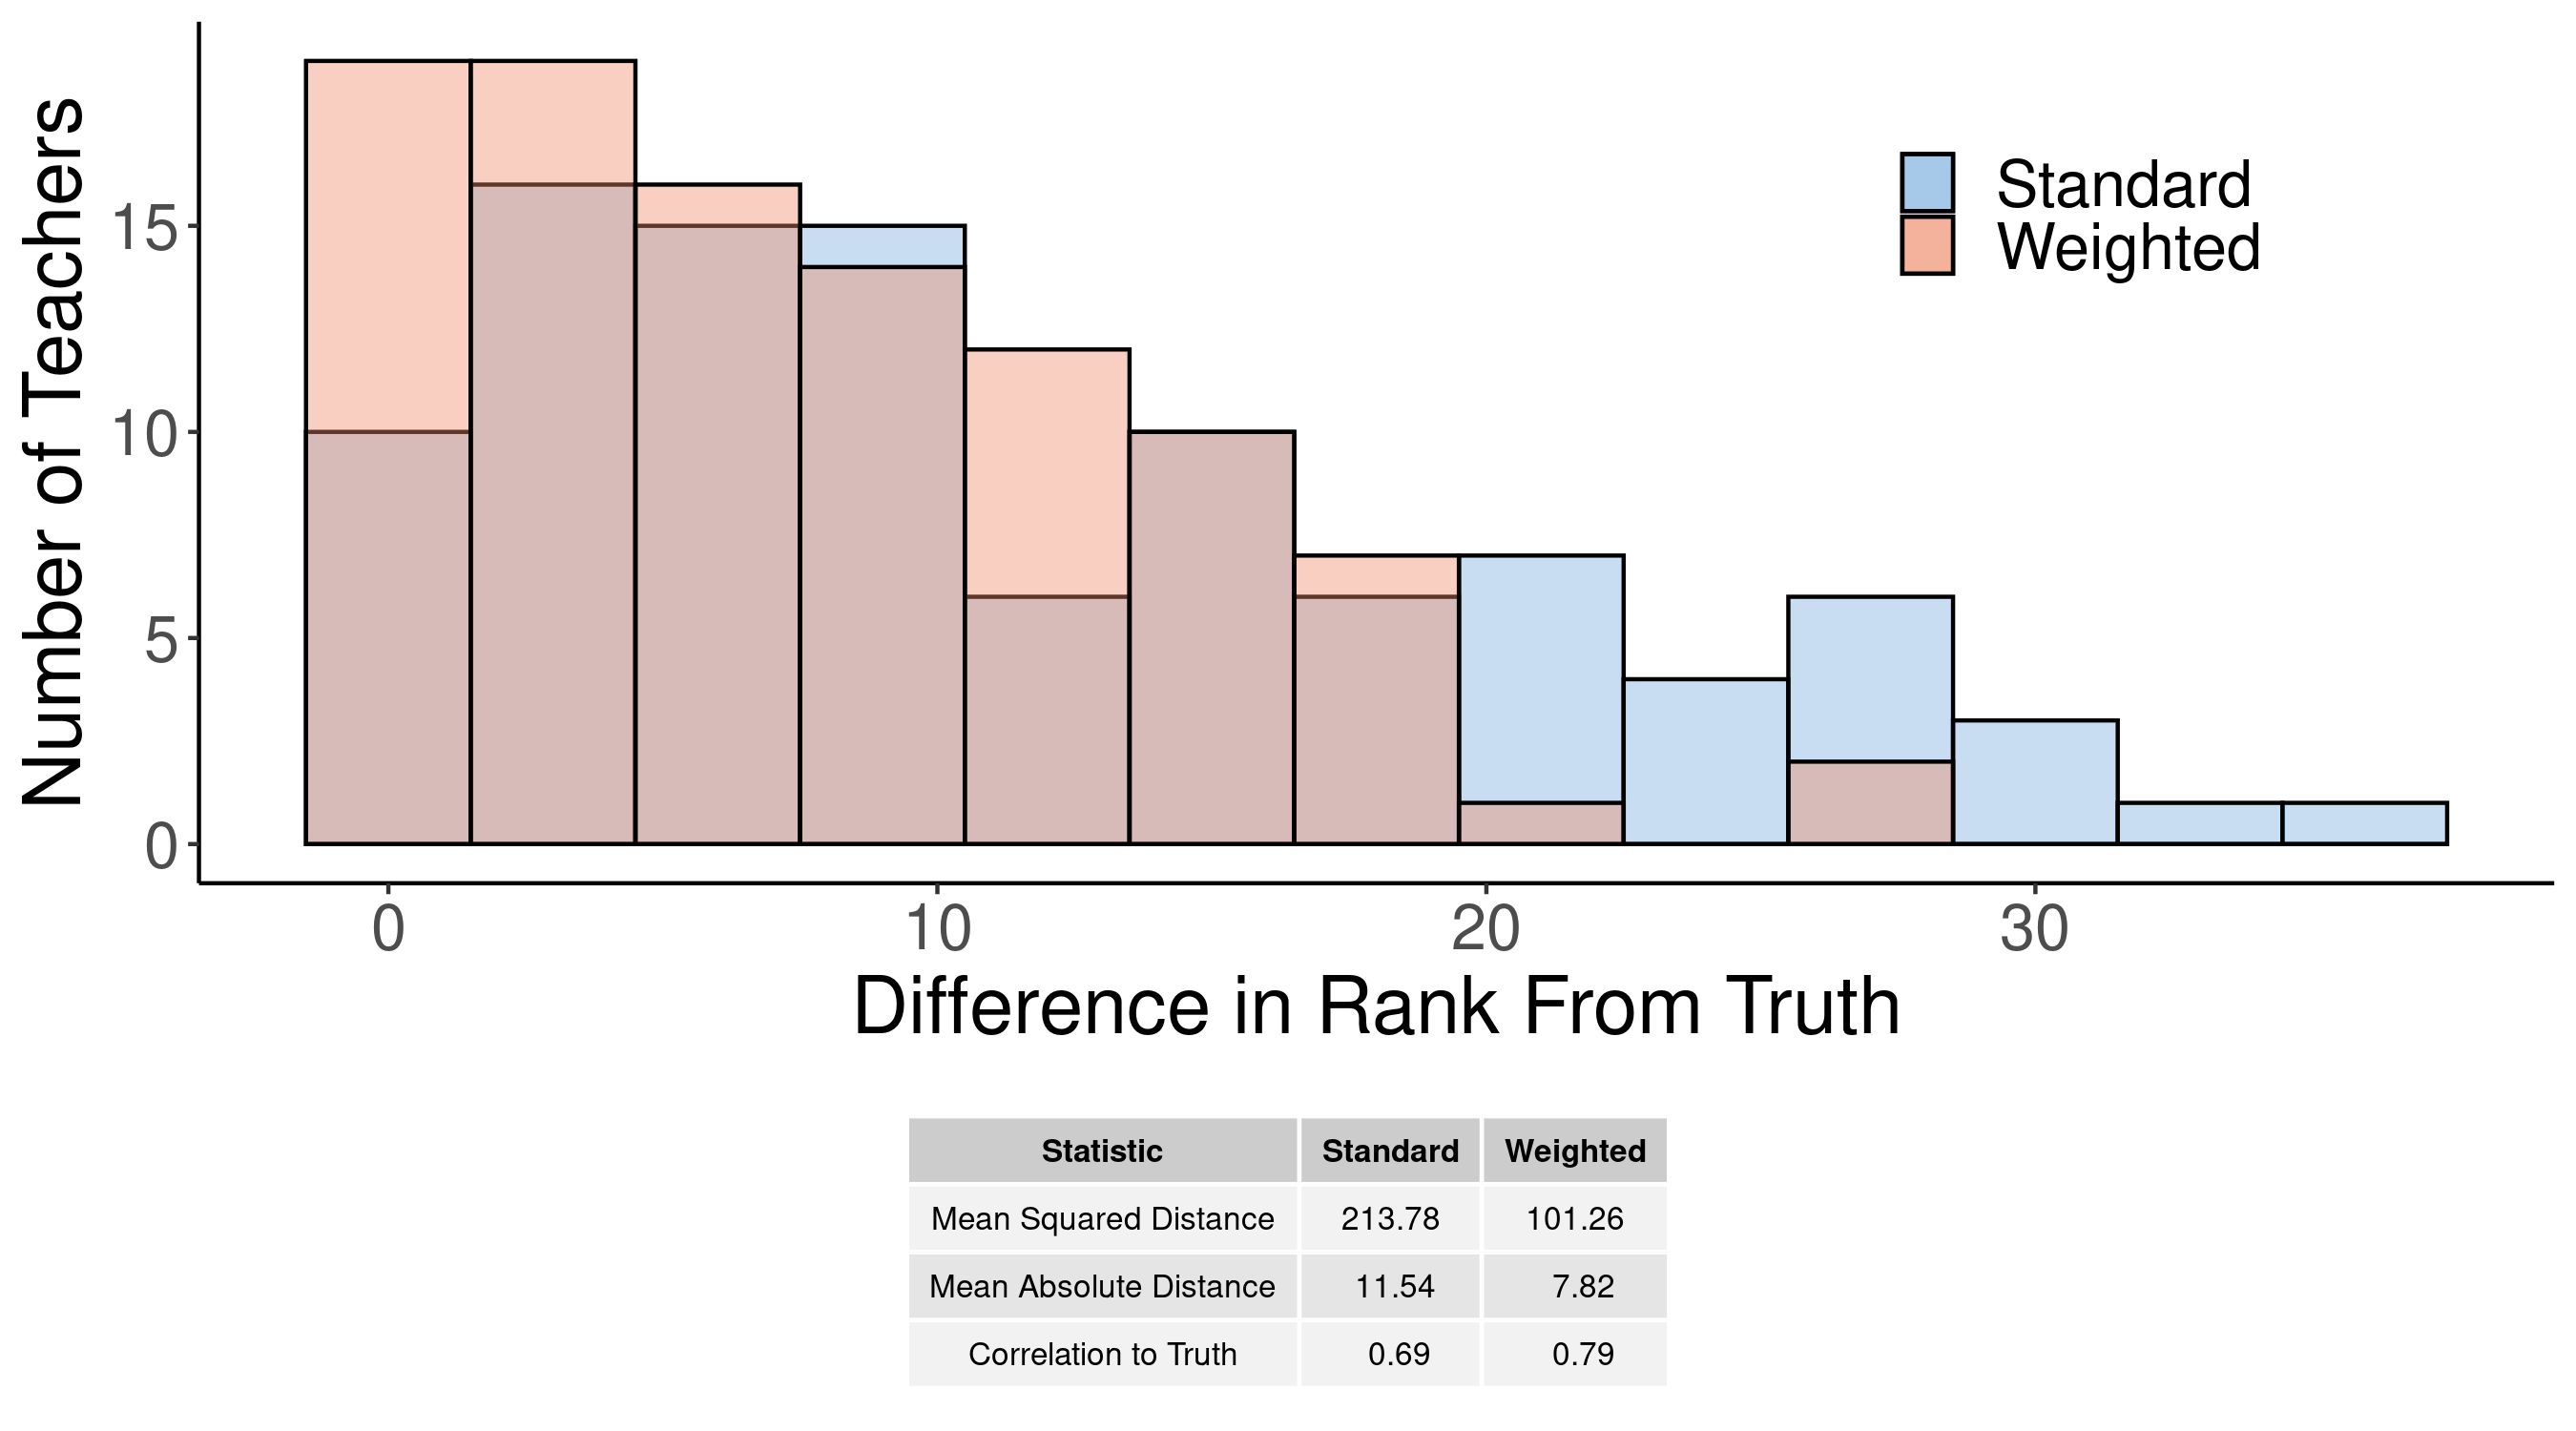
\includegraphics[width=.9\textwidth]{slides/CIERS_Figures/np_hist_run_2.png}
    \label{fig:hist}
\end{figure}





%%%%%%%%%%%%%%%%%%%%%%%%%%%%%%%%%%%%%%%%%%%%%%%%%%%%%%%%%%%%%%%%%
%%%%%%%%%%%%%%%%%%%%%%%%%% References %%%%%%%%%%%%%%%%%%%%%%%%%%%
%%%%%%%%%%%%%%%%%%%%%%%%%%%%%%%%%%%%%%%%%%%%%%%%%%%%%%%%%%%%%%%%%

\bibliography{citations}

\end{document}
